\section{Methodology}

\begin{figure*}
    \centering
    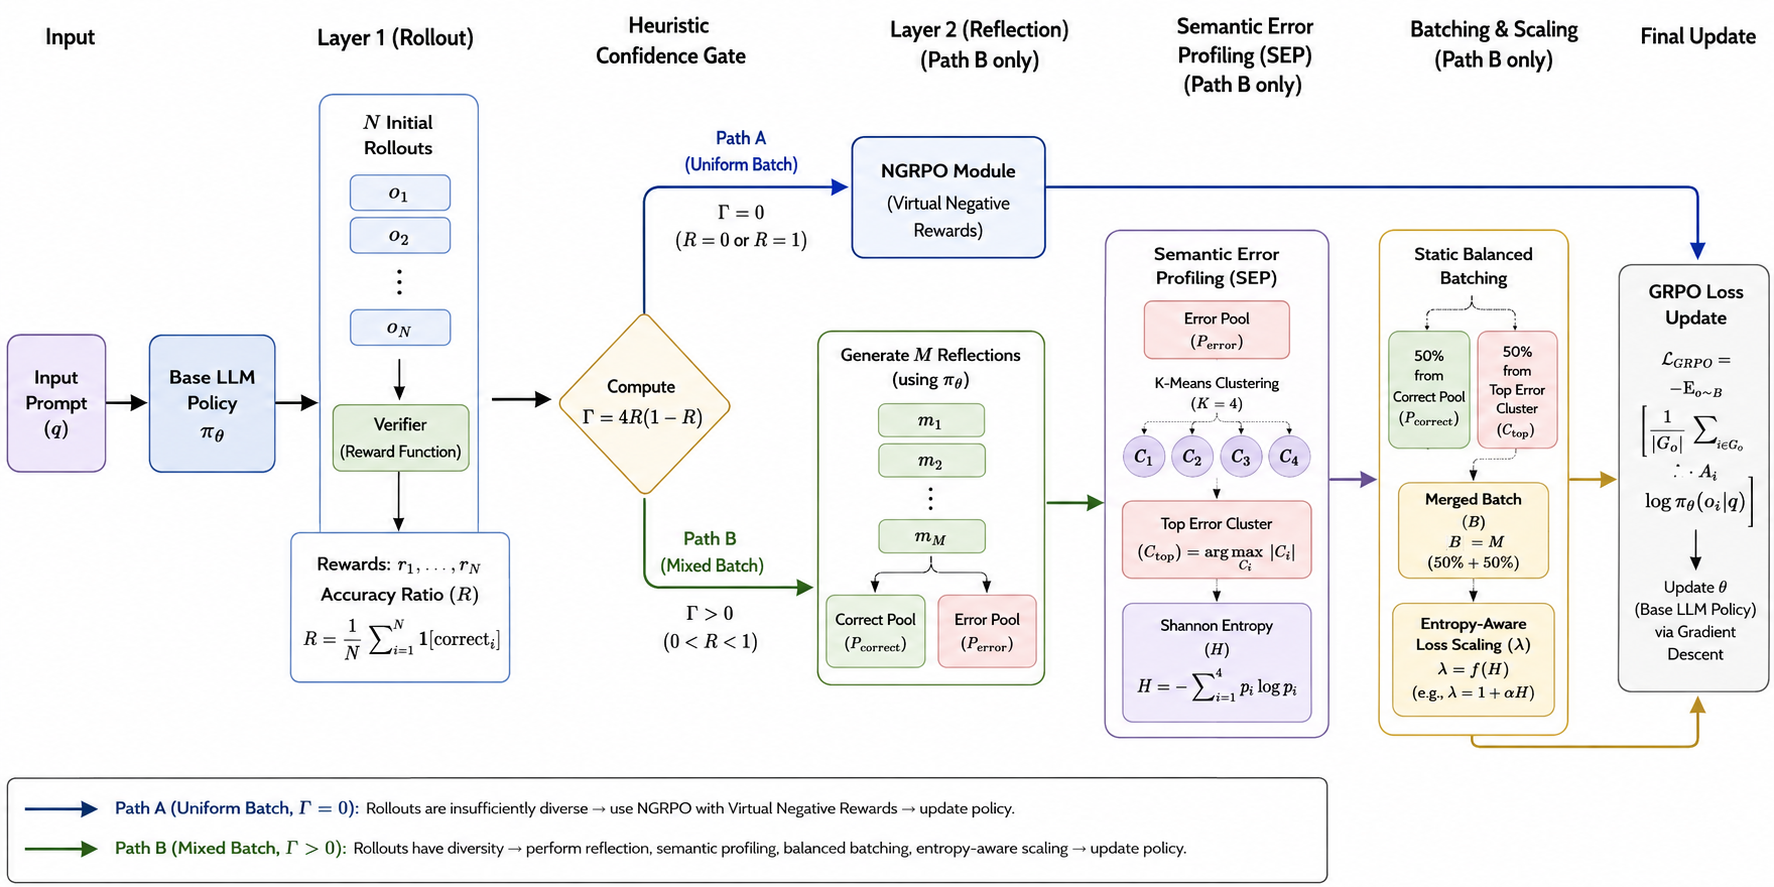
\includegraphics[width=\textwidth]{sb-grpo-diagram.png}
    \caption{The complete system architecture of SB-GRPO. The Heuristic Confidence Gate ($\Gamma$) dynamically routes uniform batches to the NGRPO module (Path A) to prevent advantage vanishing. For mixed batches (Path B), the framework applies Multi-Layer Reflection and Semantic Error Profiling (SEP) to extract the Top Error Cluster ($C_{top}$), forming a Static Balanced Batch optimized by an Entropy-Aware Loss Scaling factor ($\lambda$).}
    \label{fig:pipeline}
\end{figure*}

\subsection{Formal Derivation of SB-GRPO}
Let $q$ be a prompt and $O = \{o_1, \dots, o_N\}$ be $N$ rollouts from policy $\pi_\theta$. The standard reward for $o_i$ is $r_i \in \{0, 1\}$. In SB-GRPO, we define the accuracy ratio: $$R = \frac{1}{N} \sum_{i=1}^N r_i$$

\subsubsection{Heuristic Confidence Gate}
To maintain gradient continuity, we define a differentiable heuristic gating function $\Gamma(R)$ using the quadratic form:
\begin{equation}
\Gamma(R) = 4R(1-R)
\end{equation}
Note that $\Gamma \in [0, 1]$, reaching $0$ at $R=0$ (all wrong) or $R=1$ (all correct), and $1$ at $R=0.5$. This parabolic form ensures that purely correct or incorrect batches seamlessly switch to pure NGRPO loss, while balanced batches optimally utilize multi-layer reflection without gradient spikes. This gate selects the advantage calculation method:
\begin{equation}
A_{i} = \Gamma \cdot A_{std} + (1-\Gamma) \cdot A_{ngrpo}
\end{equation}
where $A_{ngrpo}$ uses a virtual reward $r_{virtual} = -1.0$ to inject a negative signal even when all $r_i=0$. The standard advantage is computed as $A_{std} = (r_i - \mu) / \sigma$, where $\mu$ and $\sigma$ are the mean and standard deviation of rewards within the group. When variance approaches zero, $A_{std}$ vanishes, making $A_{ngrpo}$ critical for continuous training.

\subsection{Layered Generation and Reflection}
The pipeline is split into two layers to simulate the "Internal Monologue" and "External Correction":
\begin{enumerate}
    \item \textbf{Layer 1 (Rollout):} $N=8$ samples are generated with temperature $T=0.7$ to explore the solution space.
    \item \textbf{Layer 2 (Reflection):} If $\Gamma > 0$, the model performs $M=2$ reflections per rollout using a neutral system prompt: \textit{"Review the solution logic. Only correct it if errors are found; otherwise, maintain consistency."} This creates a pool of $N \times M = 16$ reasoning paths.
\end{enumerate}

\begin{algorithm}
\caption{SB-GRPO Training Step}
\begin{algorithmic}[1]
\STATE \textbf{Input:} Prompt $q$, Policy $\pi_\theta$, Verifier $V$
\STATE Generate $N$ rollouts $O = \{o_1, \dots, o_N\}$ via vLLM
\STATE $R \gets \text{accuracy\_ratio}(O, V)$
\STATE $\Gamma \gets 4R(1-R)$
\IF{$\Gamma > 0$}
    \STATE Generate $M$ reflections per rollout $\to$ Pool $P$
    \STATE Cluster $P_{error}$ into $\{C_1 \dots C_K\}$ using K-Means
    \STATE $\lambda \gets \exp(-\text{Entropy}(C)/\tau)$
    \STATE $B \gets$ Sample $S/2$ from $P_{correct}$ and $S/2$ from $C_{top}$
\ELSE
    \STATE $\lambda \gets 1.0$, $B \gets$ Sample $S$ uniformly from $O$
    \STATE Use NGRPO Virtual Advantage $A_{ngrpo}$
\ENDIF
\STATE \textbf{Training Phase:}
\STATE Flush vLLM cache $\to$ Init PyTorch Trainer
\STATE $\rho \gets \frac{\pi_\theta}{\pi_{old}}$
\STATE $\mathcal{L}_{surr} \gets \min\left(\rho A, \text{clip}\left(\rho, 1-\epsilon, 1+\epsilon\right)A\right)$
\STATE $\mathcal{L}_{GRPO} \gets \frac{1}{|B|} \sum \lambda \left[ \mathcal{L}_{surr} - \beta \mathbb{D}_{KL} \right]$
\STATE Backward and Optimizer Step
\end{algorithmic}
\end{algorithm}

\subsection{Semantic Error Profiling (SEP)}
Incorrect samples are vectorized using a frozen \textit{all-MiniLM-L6-v2} encoder running entirely on the CPU to avoid VRAM contention. We apply K-Means clustering ($K=4$) to partition the errors into semantic clusters $C = \{C_1, \dots, C_k\}$. We identify the \textbf{Top Error Cluster} $C_{top} = \text{argmax}_k |C_k|$. This cluster represents the most common logical failure mode for the given prompt, allowing for \textbf{Targeted Error Correction}.

\subsection{Information-Theoretic Loss Scaling}
We measure the uncertainty of the model's error state via the Shannon Entropy $H$ of the cluster distribution $p_k = |C_k| / \sum |C_j|$:
\begin{equation}
H = - \sum_{k=1}^K p_k \log(p_k)
\end{equation}
The loss scaling factor $\lambda = \exp(-H/\tau)$ (where temperature $\tau=1.0$) is applied to the policy gradient. High entropy (random, diverse arithmetic errors) leads to smaller updates, while low entropy (concentrated, systematic logical errors) leads to larger updates.

\subsection{Hardware-Aware Static Tensor Shaping}
To maximize GPU throughput on NVIDIA H100 and prevent memory fragmentation caused by dynamic sequence lengths, we avoid all dynamic padding. Furthermore, taking inspiration from the DIVA-GRPO variance reduction theorem, we construct a \textbf{Static Balanced Batch} of size $S=16$. We draw $S/2$ samples from the Correct Pool and $S/2$ from $C_{top}$. \textbf{Sampling with Replacement} is used to guarantee the tensor shape is entirely constant at every step. This static configuration is hyper-optimized for maximizing DeepSpeed ZeRO-3 performance.
